%% new commands
\newcommand{\rxj}{RX J0913.7+4056}
\newcommand{\iras}{IRAS 09104+4109}
\newcommand{\irs}{I09}

%% load preferences
\documentclass[11pt]{article}
\usepackage{graphicx,common}
\usepackage[nonamebreak,numbers,sort&compress]{natbib}
\bibliographystyle{plainnat}
\setlength{\textwidth}{6.5in} 
\setlength{\textheight}{10in}
\setlength{\topmargin}{0in} 
\setlength{\oddsidemargin}{-0.13in}
\setlength{\evensidemargin}{0in} 
\setlength{\headheight}{-0.3in}
\setlength{\headsep}{0in} 
\setlength{\hoffset}{0in}
\setlength{\voffset}{0in}

%% get rid of blank line in bib
\let\oldbib=\thebibliography
\let\endoldbib=\endthebibliography
\renewenvironment{thebibliography}[1]{
  \begin{oldbib}{#1}
    \setlength{\parskip}{0pt}
    \setlength{\itemsep}{0pt}
}{\end{oldbib}}

%% start the doc
\begin{document}
\pagestyle{plain}
\pagenumbering{arabic}

\noindent{\bf{\uppercase{Scientific Justification}}}\\

Unlike most ULIRGs, \irs\ is a BCG, but unlike most BCGs, \irs\ hosts
a heavily-obscured QSO which gives rise to the enormous IR luminosity
\cite{kleinmann88, hines93, evans98}. Hines et al. \cite{hines99}
convincingly demonstrate that beamed QSO radiation is emerging from
the nucleus in a direction coincident with a photoionized, [O
  \Rmnum{3}]-dominated nebula (see Fig. \ref{fig:img}), and Cavagnolo
et al. \cite{cavagnolo10} further show that the X-ray emission
associated with this region is well-modeled as QSO irradiation of the
nebula and surrounding intracluster medium (ICM). Additionally, there
is a spur of radio emission protruding from the nucleus which is
coincident with the nucleus beaming direction. The observational
evidence strongly indicates the presence of an active nucleus with a
beaming axis directed to the NE of \irs. However, the beamed emission
is significantly misaligned with the large-scale radio jets which run
NW \& SE from the nucleus \cite{hines93, hines99}. Further, the radio
source is a peculiar borderline FR-I/II with a core spectrum which is
significantly flatter than the jets, so much so that it appears the
jets are no longer being fed by the nucleus \cite{hines93}. The beamed
nuclear radiation and jets clearly constitute two distinct physical
systems, but are their origins one in the same? Is there a single SMBH
in the nucleus which created the jets and is now beaming in a
dramatically new direction? Or could it be that the nucleus hosts
multiple SMBHs with anisotropic spin axes? Assuming SMBH spin,
beaming, and jet axes are co-aligned, the central engine of \irs\ was
re-oriented no less than 70 kyr ago \cite{hines99}, but no more than
$\sim 10$ Myr \cite{cavagnolo10} adding a further constraint on the
processes which caused the misalignment. But while understanding the
nature of the \irs\ nucleus is interesting in its own right, \irs\ is
also an important low-redshift analog of higher-redshift systems where
the majority of SMBH formation and massive galaxy/BCG assembly occurs.

Most galaxies harbor a central SMBH which likely co-evolved with the
host galaxy, giving rise to well-known correlations between bulge
luminosity, stellar velocity dispersion, and black hole mass
\cite{kormendy95, magorrian}. It is believed that a key element of the
co-evolution, in addition to mergers, is energetic feedback from
accreting SMBHs, either in a radiatively-dominated quasar-mode
\cite[\eg][]{springel05} or a kinetically-dominated radio-mode
\cite[\eg][]{croton06}. The quasar-mode is expected to be brief,
expelling large quantities of cold gas from the host galaxy, whereas
the radio-mode is prolonged \& intermittent, heating the extended hot
halo (\eg\ the ICM) such that future cooling is regulated. As
evidenced by AGN excavated cavities in X-ray halos, there are numerous
examples of systems dominated by mechanical feedback
\cite[\eg][]{fabian00}, and there are indications that many
high-redshift galaxies are dominated by QSO feedback
\cite{veilleux05}. But, in a unified feedback model, there are
expected to be ``transition'' systems which bridge the dominance of
one mode over another. \irs\ is curious because it has cavities in the
X-ray halo ($L \sim 10^{44} ~\lum$) and a powerful QSO ($L \sim
10^{47} ~\lum$), prompting Cavagnolo et al. \cite{cavagnolo10} to
suggest, among other reasons, that \irs\ is a ``transition'' system
and that the beam-jet misalignment is signaling the evolution of the
feedback mode from radiation dominance to mechanical dominance. The
implication being that we are getting a glimpse of a very short-lived
epoch of the AGN/QSO feedback cycle, and thus \irs\ provides us the
opportunity to study how SMBH evolution relates with the host
environment. But a key to advancing this understanding is further
resolving the nucleus.

Simply put, a multitude of models and explanations are possible for
the misalignment, and evaluating these models in the context of the
feedback paradigm first requires resolving the nuclear structure. For
example, rapid spin axis realignment is predicted in some black hole
merger scenarios, \eg\ the ``spin flip'' model of
\cite{merritt02}. But, rapid jet reorientation can also occur as a
result of accretion disk instabilities \cite{dennett02}. There is the
remote possibility that the beaming direction has not been altered at
all, but what we are witnessing is the jet outflow being diverted by
external pressure gradients causing a back-flow
\cite[\eg][]{worrall95}. Or, there may simply be two or more
SMBHs. Another tantalizing model is that of retrograde spin evolution
\cite{garofalo10}. In this model SMBHs are expected to pass through a
low spin state where a massive accretion flow would be capable of
rapidly changing the spin axis. But in this model, the kinetic power
output of the AGN (which we have directly estimated with the X-ray
cavities) is tied to the handedness of the SMBH spin relative to the
accreting material. The difference between these scenarios being that,
the number of nuclear sources, the synchrotron power of the accretion
disk, and the sub-kpc scale jet structures are fundamentally
different: pairs of continuous, deformed jets versus sparse,
distinctly separate jet pairs; one point source versus more than one
point source; the connection of the small-scale jets to the
large-scale jets. If we find the family of models which involve
mergers are consistent with the \irs\ nucleus, then it suggests
\irs\ is a reasonable template for similar massive galaxies. But if
the more rare processes like spin-slip or retrograde spin evolution
seem to be more appropriate, then \irs\ would seem to be an oddity in
the massive galaxy formation model.

It is also worth noting that the radio spur NE of the core does not
have a SW counter-spur. The proposed observations will reveal whether
there is a counter-jet or if the system is one-sided. This
determination will yield insight regarding the inclination of the
beaming axis. This information will be used to further constrain the
orientation and structure of obscuring nuclear material, which has
been the focus of extensive study, but with some ambiguity
\cite[\eg][]{tran00, taniguchi97}.

Additional radio observations are needed to directly image the
synchrotron emission of relativistic particles which are markers of
on-going process which are below the sensitivity and resolution limits
in other wave-bands, \ie\ X-ray, optical, and UV. While \irs\ has been
observed at the highest resolution attainable with the VLA, the
sub-arcsecond capabilities of the VLBA are needed to further probe the
nuclear structure and minimize confusion between multiple radio
sources. Technical details of our requests are discussed in the next
section.\\

\noindent{\bf{\uppercase{Technical Justification}}}\\

To determine the observational parameters needed to achieve our
scientific goals, the highest-resolution VLA images were used as a
guide and subsequent exposure times calculated using the EVN
Calculator\footnote{http://www.evlbi.org/cgi-bin/EVNcalc.pl}. The
\irs\ radio core has a flux of 1.6 mJy at 6 cm (4.9 GHz) and 5.9 mJy
at 20 cm (1.5 GHz). The VLA A-configuration observations at 6 cm
($\approx 0.4\arcs \times 0.3\arcs$ beam) and 20 cm ($\approx 1.3\arcs
\times 1.2\arcs$ beam) have respective peak flux densities of 1.0 mJy
beam$^{-1}$ and 4.6 mJy beam$^{-1}$, and both have off-axis
$\sigma_{\rm{rms}}$ of $\approx 35 ~\mu$Jy beam$^{-1}$. We find that
for a VLBA setup with 2 polarizations, 4 sub-bands per polarization,
and 8 MHz of bandwidth, an integration time of 360 min will result in
image thermal noise ($1\sigma$; natural weighting) of $\approx 38
~\mu$Jy beam$^{-1}$ for L-band (21 cm) and $\approx 40 ~\mu$Jy
beam$^{-1}$ for C-band (6 cm) with an aggregate bit rate of 256 Mbps
(2 bit sampling). This is comparable to the VLA noise levels which
resulted in high-quality imaging. The maximum half-power beam-widths
will be $\approx 5.0$ mas at 21 cm and $\approx 1.4$ mas at 6 cm, with
respective time-smearing limited field-of-views (FOVs) of $10.8\arcs$
and $3.1\arcs$ (shown in Fig. \ref{fig:img}). For a \cosmo, these
resolutions equate to 30 pc at 21 cm and 8 pc at 6 cm. The requested
observations are sufficient to yield $3\sigma$ detections of sources
with fluxes $\ga 1$ mJy and obviously resolve structures separated by
$\ga 10$ pc. Observing \irs\ during two 6 hr sessions will ensure
excellent $uv$ coverage and sufficiently deep observations to yield
reliable imaging of the rich GHz intensity structure.\\

\clearpage
{\def\section*#1{}
  \begin{thebibliography}{100}
  \bibitem{cavagnolo10} Cavagnolo et al. submitted to MNRAS, 2010.
  \bibitem{crawford96} Crawford \& Vanderriest. MNRAS, 283:1003--1014, 1996.
  \bibitem{croton06} Croton et al. MNRAS, 365:11--28, 2006.
  \bibitem{deane01} Deane \& Trentham. MNRAS, 326:1467--1474, 2001.
  \bibitem{dennett02} Dennett-Thorpe et al. MNRAS, 330:609--620, 2002.
  \bibitem{donahue93} Donahue \& Voit. ApJ, 414:L17--L20, 1993.
  \bibitem{evans98} Evans et al. ApJ, 506:205--221, 1998.
  \bibitem{fabian00} Fabian et al. MNRAS, 318:65--68, 2000.
  \bibitem{garofalo10} Garofalo et al. arXiv:1004.1166, 2010.
  \bibitem{hines93} Hines \& Wills. ApJ, 415:82-+, 1993.
  \bibitem{hines99} Hines et al. ApJ, 512:145--156, 1999.
  \bibitem{kleinmann88} Kleinmann et al. ApJ, 328:161--169, 1988.
  \bibitem{kormendy95} Kormendy \& Richstone. ARA\&A, 33:581-+, 1995.
  \bibitem{magorrian} Magorrian et al. AJ, 115:2285--2305, 1998.
  \bibitem{merritt02} Merritt \& Ekers. Science, 297:1310--1313, 2002.
  \bibitem{peeters04} Peeters et al. ApJ, 613:986--1003, 2004.
  \bibitem{sargsyan08} Sargsyan et al. ApJ, 683:114--122, 2008.
  \bibitem{springel05} Springel et al. Nature, 435:629--636, 2005.
  \bibitem{taniguchi97} Taniguchi et al. A\&A, 318:1-4, 1997.
  \bibitem{tran00} Tran et al. AJ, 120:562--574, 2000.
  \bibitem{worrall95} Worrall et al. ApJ, 449:03-+, 1995.
  \bibitem{veilleux05} Veilleux et al. ARA\&A, 43:769--826, 2005.
  \end{thebibliography}
}

\clearpage
\begin{figure}[htp]
  \begin{center}
    \begin{minipage}{0.63\linewidth}
      \includegraphics[width=\textwidth]{vla.ps}
    \end{minipage}
    \begin{minipage}{0.6\linewidth}
      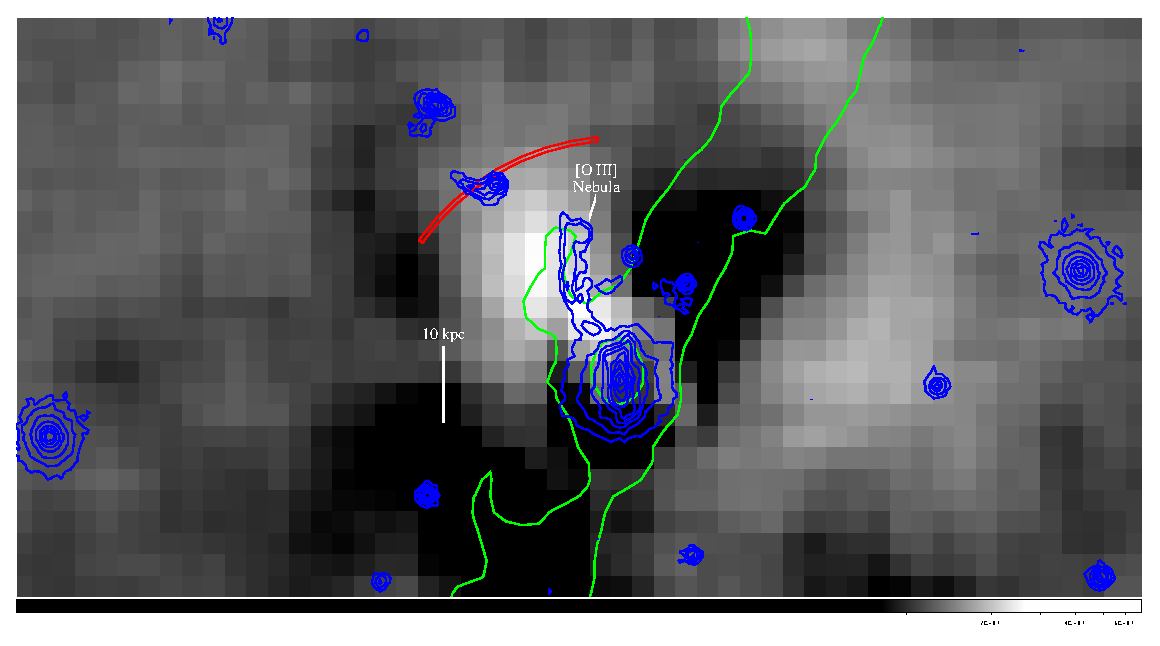
\includegraphics[width=\textwidth, trim=66mm 25mm 70mm 18mm, clip]{opt_xray.ps}
    \end{minipage}
    \caption{{\it{Left}}: 20 cm VLA A-configuration image in
      mJy. Green contours trace 20 cm emission, dashed white circles
      denote VLBA FOVs, dashed yellow vector is semi-major axis of
      \rxj, and red vectors bound QSO beaming direction. {\it{Right:}}
      X-ray image of \rxj\ core after subtracting off ICM
      emission. Green contours are lowest and highest significance 20
      cm emission, blue contours are optical emission, and red wedge
      marks the extent of scattered UV emission.}
    \label{fig:img}
  \end{center}
\end{figure}

\end{document}
